% Standalone source for the paper figure; build with figures/build.sh
\documentclass[border=1pt]{standalone}
% Shared preamble for the standalone figure sources.
\usepackage{times}
\usepackage{amsmath,amssymb}
\usepackage{xcolor}
\usepackage{textcomp}
\usepackage{tikz}
\usepackage{pgfplots}
\usetikzlibrary{arrows.meta,positioning,calc,fit,backgrounds}
\usepgfplotslibrary{fillbetween}
\pgfplotsset{compat=1.16}

% Colours are colour-blind safe (Okabe--Ito) and every figure also separates
% its classes by line style or fill, so the figures stay readable in greyscale.
\definecolor{cObs}{HTML}{0072B2}   % observed by the network
\definecolor{cHid}{HTML}{D55E00}   % hidden / unexplained
\definecolor{cHelp}{HTML}{009E73}  % safety helpers
\definecolor{cInk}{HTML}{333333}

\tikzset{
  box/.style={draw=cInk!70, rounded corners=1.5pt, fill=white, align=center,
              font=\scriptsize, inner sep=3pt, minimum height=0.8cm,
              line width=0.5pt},
  obs/.style={box, draw=cObs, fill=cObs!8},
  hid/.style={box, draw=cHid, fill=cHid!10},
  help/.style={box, draw=cHelp, fill=cHelp!10},
  flow/.style={-{Stealth[length=4pt]}, line width=0.6pt, draw=cInk!80},
  lbl/.style={font=\scriptsize, text=cInk!85, inner sep=1.5pt, align=center},
}
\pgfplotsset{
  every axis/.append style={font=\scriptsize, tick label style={font=\scriptsize},
                            label style={font=\scriptsize},
                            title style={font=\scriptsize\bfseries}, line width=0.5pt},
}

\begin{document}
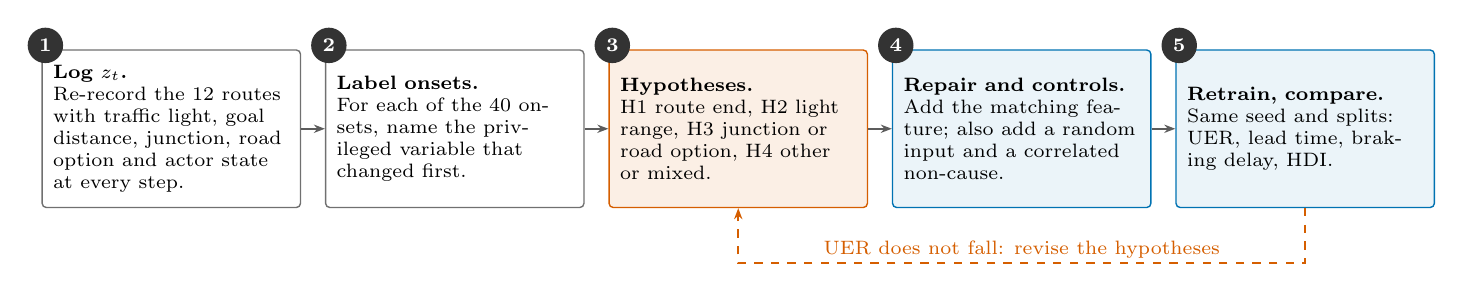
\begin{tikzpicture}[x=1cm,y=1cm]
\tikzset{pbox/.style={text width=3.0cm, minimum height=2.0cm, align=left,
                      inner sep=4pt},
         num/.style={circle, fill=cInk, text=white, font=\scriptsize\bfseries,
                     inner sep=1.5pt, minimum size=0.45cm}}
\node[box, pbox] (s1) at (0,0)
  {\textbf{Log $z_t$.}\\ Re-record the 12 routes with traffic light, goal
   distance, junction, road option and actor state at every step.};
\node[box, pbox] (s2) at (3.6,0)
  {\textbf{Label onsets.}\\ For each of the 40 onsets, name the privileged
   variable that changed first.};
\node[hid, pbox] (s3) at (7.2,0)
  {\textbf{Hypotheses.}\\ H1 route end, H2 light range, H3 junction or road
   option, H4 other or mixed.};
\node[obs, pbox] (s4) at (10.8,0)
  {\textbf{Repair and controls.}\\ Add the matching feature; also add a
   random input and a correlated non-cause.};
\node[obs, pbox] (s5) at (14.4,0)
  {\textbf{Retrain, compare.}\\ Same seed and splits: UER, lead time,
   braking delay, HDI.};
\foreach \a/\b in {s1/s2,s2/s3,s3/s4,s4/s5}
  \draw[flow] (\a.east) -- (\b.west);
\foreach \s/\n in {s1/1,s2/2,s3/3,s4/4,s5/5}
  \node[num] at ($(\s.north west)+(0.05,0.05)$) {\n};
\draw[flow, dashed, draw=cHid] (s5.south) -- ++(0,-0.7) -|
  node[lbl, pos=0.25, above, text=cHid] {UER does not fall: revise the hypotheses} (s3.south);
\end{tikzpicture}
\end{document}
